\chapter{Testing}


Have you ever had a situation when your software has a bug but it is
not discovered for a long time?  The existence of the bug and its
ability to escape detection may surprise your entire team. ``How did
that happen?'', you may ask.  This may happen due to a wide variety of
reasons. One of the possible reasons is that the software has not been
well tested and as a result the bug is not detected. Testing is an
important method detecting bugs.  However, testing can be tideous.  It
is common that someone makes a ``small'' change and skips testing.
The person believes the change is so small and cannot possibly have
any bug.  If several people add a few small changes here and there,
the software soon is full of ``small'' bugs.  Why do people not test
their programs immediately after they have made changes?  One reason
is that testing require additional work.

Is it possible testing is fully automated without any additional
effort? {\it Continuous Integration} (CI) does exactly that.

You still need to write testers. There is no way avoiding that part.
What continuous integration does is to automatically invole these
testers whenver you push your program to the shared repository.
This chapter uses {\tt Travis-CI} for continuous integration. Before explaining how
to use Continuous Integration, it is necessary first explaining how Python
testing works.

\section{Limitations of Testing}

It is important understanding that testing has limitations.  It is
practically impossible testing every possible scenario.  Every {\tt
  if} is a {\it condition}. A condition divides a program into two
different paths depending whether the condition is true or not.  A
non-trivial program can easily have hundreds of conditions.  As a
simple explanation why it is not possible testing every possible
scenario. Let's consider a program with 100 {\it independent}
conditions, i.e., whether condition is true or false does not affect
any other condition.  There are $2^{100}$ possible scenarios.  The
fastest computer in the world can perform several hundred quadrillion
($10^{15}$) calculations per second; this is a parallel computer but
let's not worry about that detail.  Because $\log_2(10) \approx 3.3$,
$10^{15} \approx 2 ^ {50}$. Thus, the fastest computer can check as
many as $2 ^ {50}$ conditions per second. How many can this computer
check per minute? $2 ^ {50} \times 60$. How about a day (86,400
seconds)?  $2 ^ {50} \times 86400 \approx 2 ^ {66}$.  In order to test
$2^{100}$ possible scenarios, this computer needs to work $2^{34}$
days; this is very long time (much longer than the history of humans).
In fact, the situation is even worse.  The estimation above considers
only two possible cases for each condition: true or false. If the
condition compares two numbers, then ``every possible scenario'' means
every possible pairs of these two numbers.  What does this mean? It
would be completely impossible testing every possible scenario of a
program's execution paths controlled by the conditions.

Does this mean there is no need to test because it is not possible
testing all possible scenarios? No. What it means is that testing has to
be done carefully so that testing can detect as many problems (i.e.,
bugs) as possible.  Good tests should consider many different scenarios.

\section{Structure of Tests}

Many books talk about the importance of testing and how to write
tests.  However, few books talk about how to structure tests. Before
writing any test, you need to answer an important question: do you
want the testing code to be sent to the users (or customers)? In most
cases, the answer is no.  The program used to generate the product
sent to customers is often called the ``production code''.  You do not
want to include test code inside production code for many reasons.
First, including testing code may make your product bigger (in terms
of storage) and slower (in terms of execution time). Worse, testing
often needs specific inputs and the expected outputs for these test
cases.  Will you also give these inputs and outputs to your customers?
If you do not, why do you include testing code in the product?

Mixing production code and testing code is a common mistake for
beginning software developers. Worse, many of them have a lot of
``debugging messages'' as they test  code. When the program is
ready for production and release, what will they do with these
debugging messages?  In almost all cases, your customers do not
understand the debugging messages and you have to remove the code
printing these messages.  Here is the problem. When you remove the
code printing these messages, the risk is too high for one of two
things to happen. First, you do not remove all the code printing the
debugging messages.  Your customers are annoyed by the mysterious
debugging messages. Your competitors know more than what you to reveal
about your proudct.  The second scenario is worse.  You accidentally
remove more code than you intend and you actually add bugs to your
program.  Your program no longer works and your customers are very
angry at your product.

The correct way of creating tests is to separate testing code from the
production code in different files (probably in different
directories).  The production code does what it needs to do
as the product. The
testing code tests the production code.  When your product is ready,
exclude the testing code, the inputs, and the expected outputs before
releasing your product.  Figure~\ref{fig:teststructure01} illustrates
this concept.

\begin{figure}[h] \centering
{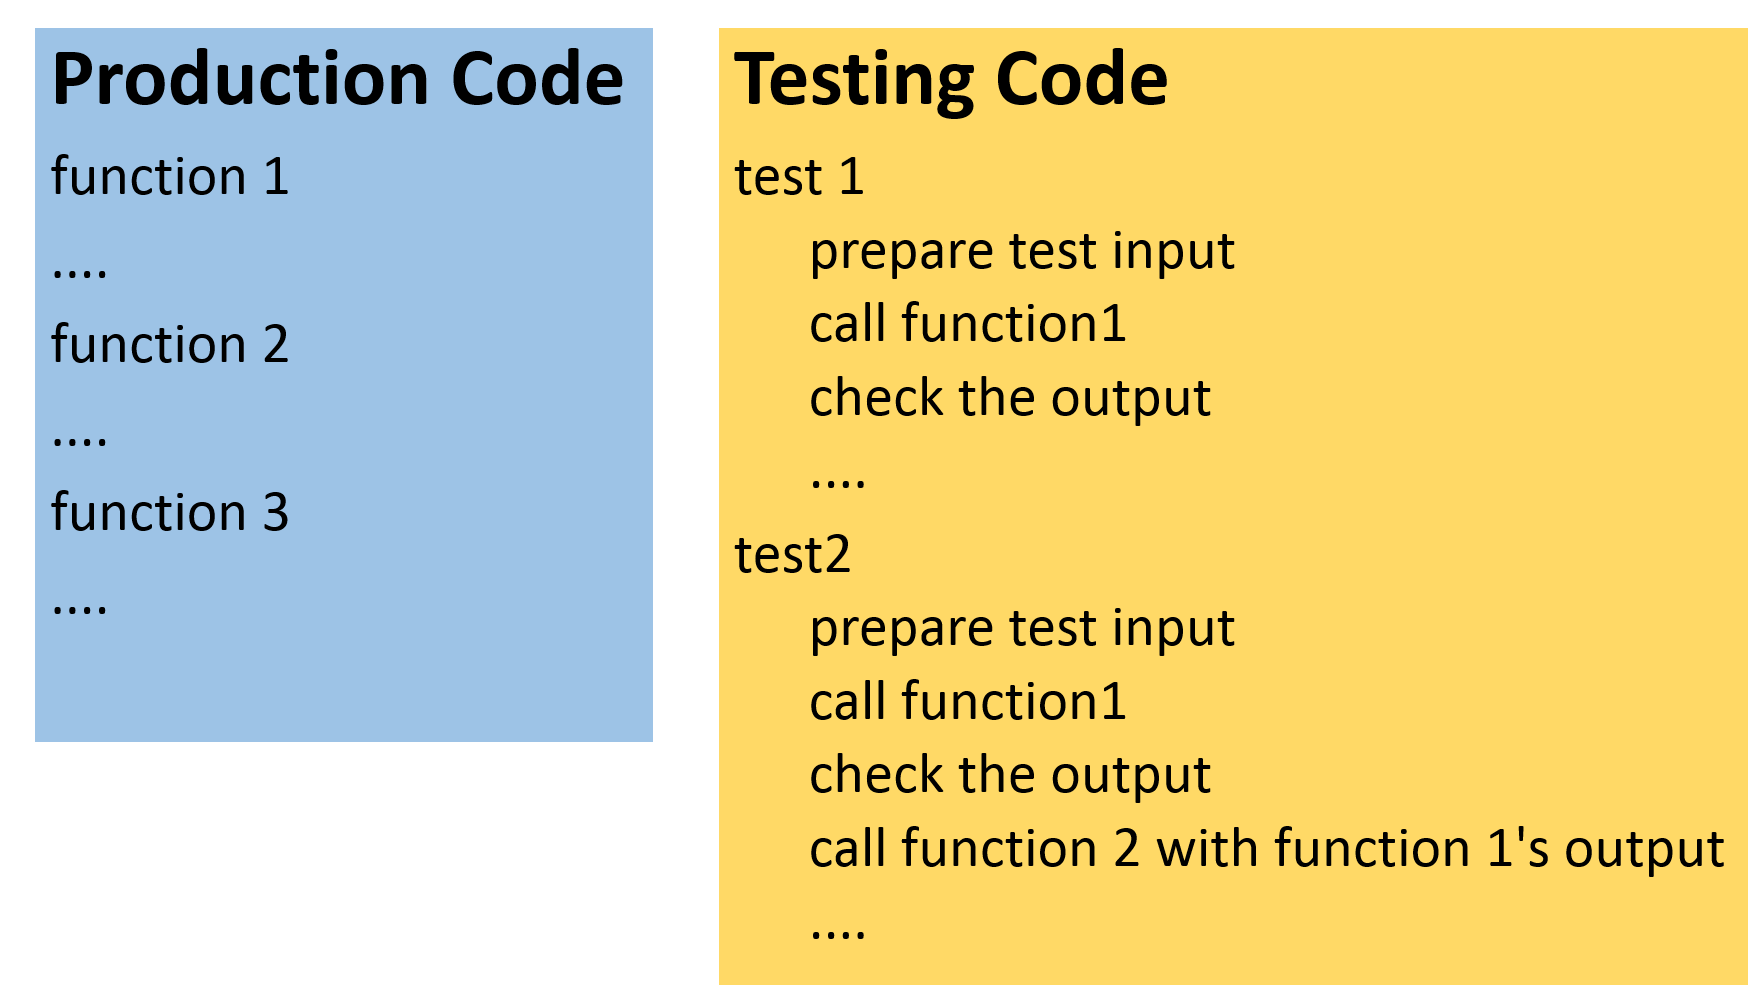
\includegraphics[width=4.5in]{\thischapterpath/figures/teststructure01.png}}
\caption{Production code and test code should be completely separated.}
\label{fig:teststructure01}
\end{figure}

\index{assert|(}
\section{Use {\tt Assert} Correctly}

Another common mistake among beginning software developers is to use
{\tt assert} incorrectly. This is what they often do.

\marginnote{These problems about misuse {\tt assert} were observed
  in the authors' classes.  They actually happened multiple times.}

\vspace{0.2in}

\noindent
\begin{tabular}{|p{5in}|}\hline
\begin{verbatim}
  # This is production code
  ....
  assert(condition that should be true)
  ....
\end{verbatim}
\\ \hline
\end{tabular}
\vspace{0.2in}

This is one example how {\tt assert} may be used:

\vspace{0.2in}

\noindent
\begin{tabular}{|p{5in}|}\hline
\begin{verbatim}
def func(x):
    assert (x > 1)
\end{verbatim}
\\ \hline
\end{tabular}
\vspace{0.2in}

There are three problems when you do this.  First, if the condition is
not true, the program {\it immediately} stops.  There is no second
chance.  Imagine that your program is a text editor. When a user wants
to save the content to a file, your program does not want to erase an
existing file.  You put {\tt assert} there claiming that the file must
not exist. If a user accidentially uses a file whose name already
exists, the program stops and everything typed by the user is lost.
You will definietely have a user that will never buy any product from
you.  Some people argue that ``I put {\tt assert} there because I know
it must be true.'' That argument is self-contraditory.  If you know
that the condition must be true, you will not put {\tt assert} there.
Would you write

\vspace{0.2in}

\noindent
\begin{tabular}{|p{5in}|}\hline
\begin{verbatim}
assert (1 > 0)
\end{verbatim}
\\ \hline
\end{tabular}
\vspace{0.2in}

You don't.

If you are abosolutly certain the condition must be true, you do not
need to put {\tt assert} there.

Some people say, ``I will remove all {\tt assert} before releasing the
product.''  This can be done easily using the {\tt grep -v} command.
This, however, brings the second problem.  What would happen if
some of the {\tt assert} statements actually do something useful?
Consider the following case:

\index{grep}


\vspace{0.2in}

\noindent
\begin{tabular}{|p{5in}|}\hline
\begin{verbatim}
assert (x = y)
\end{verbatim}
\\ \hline
\end{tabular}
\vspace{0.2in}

This assigns {\tt y}'s value to {\tt x}.

What you really want to do is probably to ensure that  {\tt x} and {\tt y}
are the same:

\vspace{0.2in}

\noindent
\begin{tabular}{|p{5in}|}\hline
\begin{verbatim}
assert (x == y)
\end{verbatim}
\\ \hline
\end{tabular}
\vspace{0.2in}

The earlier {\tt assert} statement assigns {\tt y}'s value to {\tt
  x}. Hence, their values are same and the intended {\tt assert} is
actually true.  If you remove the {\tt assert} and no longer assign
{\tt y}'s value to {\tt x}, the program may not work any more. Human
eyes are not good detecting the differences between {\tt =} and {\tt
  ==}. This is a difficult bug to fix because keeping {\tt assert}
means the program is correct. Removing {\tt assert} means the program
is wrong.


\marginnote{Do not put {\tt assert} in your production code.}

The third problem is, perhaps, somewhat philosophical.  It is the
attitude of creating good software.  Software is deployed in many
safety-critical systems. Mistakes in these systems may cause
signficant amounts of financial losses, body injuries, or even deaths.
Allowing a program to sudden stop is simply an unacceptable way of
thinking.  Using {\tt assert} is an {\it irresponsible} way of writing
production code.  It expresses the attutide ``Something is not
expected. My program commits suicide and the rest is not my problem
any more.''  A more responsbile way of writing good software is to
{\it handle the problem and do not stop the program}.

If {\tt assert} has these problems, does that mean {\tt assert} should
not be used at all?  You should not use {\tt assert} in production
code.  You can use {\tt assert} in the testing code, as shown in
Figure~\ref{fig:teststructure02}.


\begin{figure}[h] \centering
{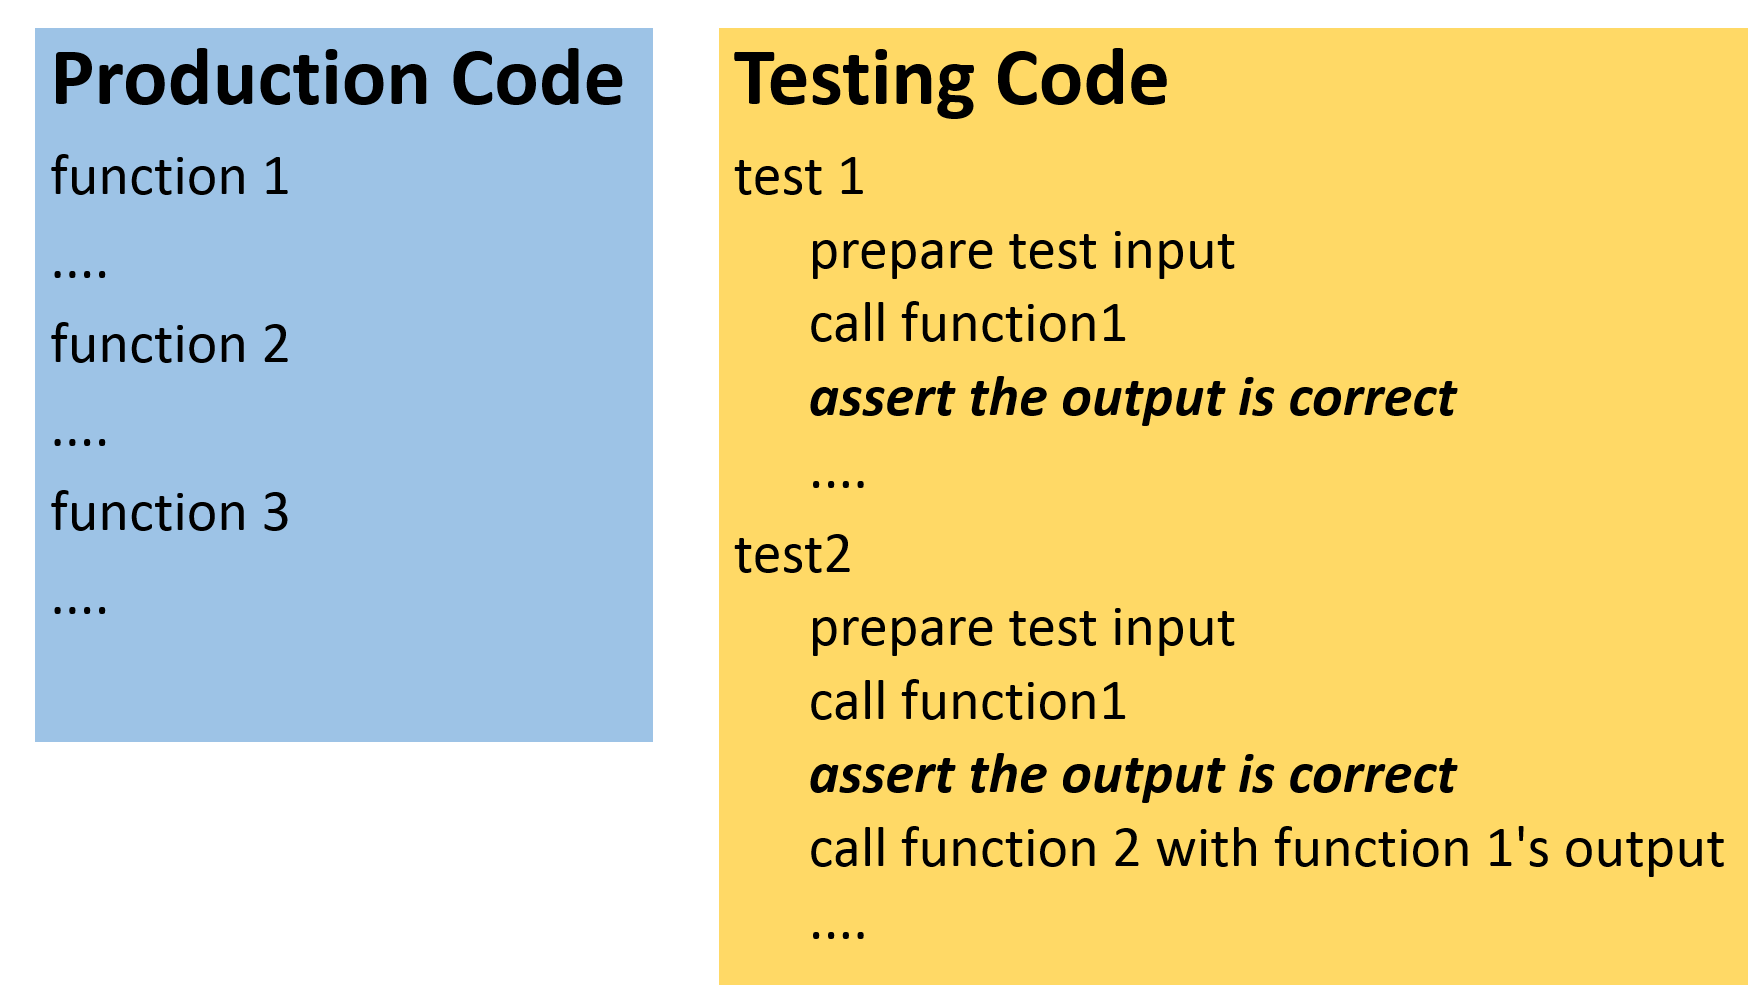
\includegraphics[width=4.5in]{\thischapterpath/figures/teststructure02.png}}
\caption{Use {\tt assert} in the testing code.}
\label{fig:teststructure02}
\end{figure}

In this example, the testing code uses {\tt assert} to check whether
the output from function 1 is correct.  This is particularly important
before sending it to the input of function 2.  This further emphasizes
the importance of separating production code from testing code.

\index{assert|)}

\section{Exception}

\index{pytest|(}
\section{Pytest}

Python has a tool for testing calle {\tt pytest}. It automatically
looks for the files starting with {\tt test\_} and ending with {\tt
  .py} and executes the functions whose names start with {\tt test\_}.
The following is a simple example.


\resetlinenumber[1]
\linenumbers
\begin{tt}
  \lstinputlisting{\progpath/software/test/test_example1.py}
\end{tt}
\nolinenumbers

Running {\tt pytest} gets the following output:

\vspace{0.2in}

\noindent
\begin{tabular}{|p{5in}|}\hline
\begin{verbatim}
$ pytest
============ test session starts =============
platform linux -- Python 3.5.2, pytest-4.3.0, py-1.8.0, pluggy-0.9.0
rootdir: /..., inifile:
collected 1 item

test_example1.py .                                
\end{verbatim}
\\ \hline
\end{tabular}
\vspace{0.2in}

Here, the {\tt rootdir} is the directory where you run {\tt pytest}.
This output means the tests have passed.

Change the program  as follows: {\tt returntrue} returns {\tt False}
and {\tt returnfalse} returns {\tt True}:

\resetlinenumber[1]
\linenumbers
\begin{tt}
  \lstinputlisting{\progpath/software/test/test_example2.py}
\end{tt}
\nolinenumbers

Running {\tt pytest} gets this result, showing the test has failed.


\vspace{0.2in}

\noindent
\begin{tabular}{|p{5in}|}\hline
\begin{verbatim}
======================== FAILURES ========================
____________________ test_truefalse ______________________

    def test_truefalse():
>       assert returntrue() == True
E       assert False == True
E        +  where False = returntrue()

test_example2.py:11: AssertionError
==================== 1 failed in 0.04 seconds ====================
\end{verbatim}
\\ \hline
\end{tabular}
\vspace{0.2in}

\marginnote{A test is useless if it can never fail.}

When you create tests, it is important that you check whether the
tests may fail. Passing tests is not the purpose of testing.  The
purpose of testing is to detect mistakes in production code and
correct the code.  If a test can never fail, this test is useless.

Next, considers a slightly more complex program for testing two
functions: {\tt f1} and {\tt f2}:

\resetlinenumber[1]
\linenumbers
\begin{tt}
  \lstinputlisting{\progpath/software/test/test_example3.py}
\end{tt}
\nolinenumbers

This is the output of {\tt pytest}:

\vspace{0.2in}

\noindent
\begin{tabular}{|p{5in}|}\hline
\begin{verbatim}
======================== FAILURES ========================
_______________________ test_f1f2 ________________________

    def test_f1f2():
        assert f1(3) == 4
        assert f1(-3) == -2
>       assert f2(3) == 4
E       assert 2 == 4
E        +  where 2 = f2(3)

test_example3.py:13: AssertionError
\end{verbatim}
\\ \hline
\end{tabular}
\vspace{0.2in}

The result says that calling {\tt f1(3)} and {\tt f1(-3)} have passed
the tests. Calling {\tt f2(3)} has failed because {\tt f2(3)}
return 2 but the test program expects 4.

Earlier this chapter said testing code and production code should be
separated. The examples for {\tt pytest} above violated this rule.
The following examples will follow the rule separating the testing
code from the tested code. Consider a file with two functions: {\tt
  f1} and {\tt f2}:

\resetlinenumber[1]
\linenumbers
\begin{tt}
  \lstinputlisting{\progpath/software/test/funcs.py}
\end{tt}
\nolinenumbers

This is the output when calling the functions interactively:

\vspace{0.2in}

\noindent
\begin{tabular}{|p{5in}|}\hline
\begin{verbatim}
$ python3
Python 3.5.2 (default, Nov 12 2018, 13:43:14) 
[GCC 5.4.0 20160609] on linux
Type "help", "copyright", "credits" or "license" for more information.
>>> import funcs
>>> funcs.f1(3)
4
>>> funcs.f2(5)
6
25
15
\end{verbatim}
\\ \hline
\end{tabular}
\vspace{0.2in}

A test program calls {\tt funcs.f1(3)} and {\tt funcs.f2(5)}.

\resetlinenumber[1]
\linenumbers
\begin{tt}
  \lstinputlisting{\progpath/software/test/test_example4.py}
\end{tt}
\nolinenumbers

Running {\tt pytest}, however, has no output. What is happening?
Instead of printing to a computer screen (also called the {\it
  console}), {\tt pytest}, captures the output.  The reason is that
{\tt pytest} does not want to print too many things.  If too many
things are printed to the screen, it is likely that some important
messages are ignored. Another reason is that {\tt pytest} often runs
automatically when no human is watching (more details about this
later in the section on Continuous Integration).
There are two solutions: The first is to tell
{\tt pytest} to print to the screen by adding {\tt -s} after {\tt
  pytest}.  This defeats the purpose of {\tt pytest}'s intention not
to print to the screen.

\index{pytest|-s}

The second is a better and more general solution: it saves the
captured output to a file. It is actually quite straightforward:

\resetlinenumber[1]
\linenumbers
\begin{tt}
  \lstinputlisting{\progpath/software/test/test_example5.py}
\end{tt}
\nolinenumbers

\index{console}

The function {\tt test\_f1f2) has an input for capturing the outputs.
  This input will be provided automatically by {\tt pytest}.  To get
  the captured output, it calls {\tt readouterr()}.  This function
  returns the captured output to standard output (also called {\tt
    stdout}) and the standard error (also called {\tt stderr}).
  Separating {\tt stdout} from {\tt stderr} gives more flexibility:
  the former is the normal output and the latter is the error
  messages.  By default, both {\tt stdout} and {\tt stderr} are shown
  on a computer screen but it is possible saving them to different
  files.

  The testing program {\tt test\_example5.py} saves the standard
  output to a file called {\tt capturedstdout}. All outputs by the
  {\tt print} statements in {\tt funcs} are saved in this file.
  The content of the file is (as expected)

 
\vspace{0.2in}

\noindent
\begin{tabular}{|p{5in}|}\hline
\begin{verbatim}
4
6
25
15
\end{verbatim}
\\ \hline
\end{tabular}
\vspace{0.2in}

When the outputs are saved to a file, testing can be done automatically
without human watching by following these steps:

\begin{enumerate}[noitemsep,nolistsep]
\item write the expected output to a file
\item capture the output from {\tt pytest} and save it to another file
\item compare the two files
\end{enumerate}

The following program shows these steps

\resetlinenumber[1]
\linenumbers
\begin{tt}
  \lstinputlisting{\progpath/software/test/test_example6.py}
\end{tt}
\nolinenumbers

The tests uses {\tt filecmp.cmp} to compare the context of two files.
As explained, if a test cannot fail, it is useless. If {\tt
  funcs.f2(5)} is replaced by {\tt funcs.f2(4)}, {\tt pytest} fails.
This suggests that {\tt pytest} is actually testing {\tt funcs.f2}.

\section{Test Integer Partition}



\section{Continous Integration}

\begin{figure}[h] \centering
{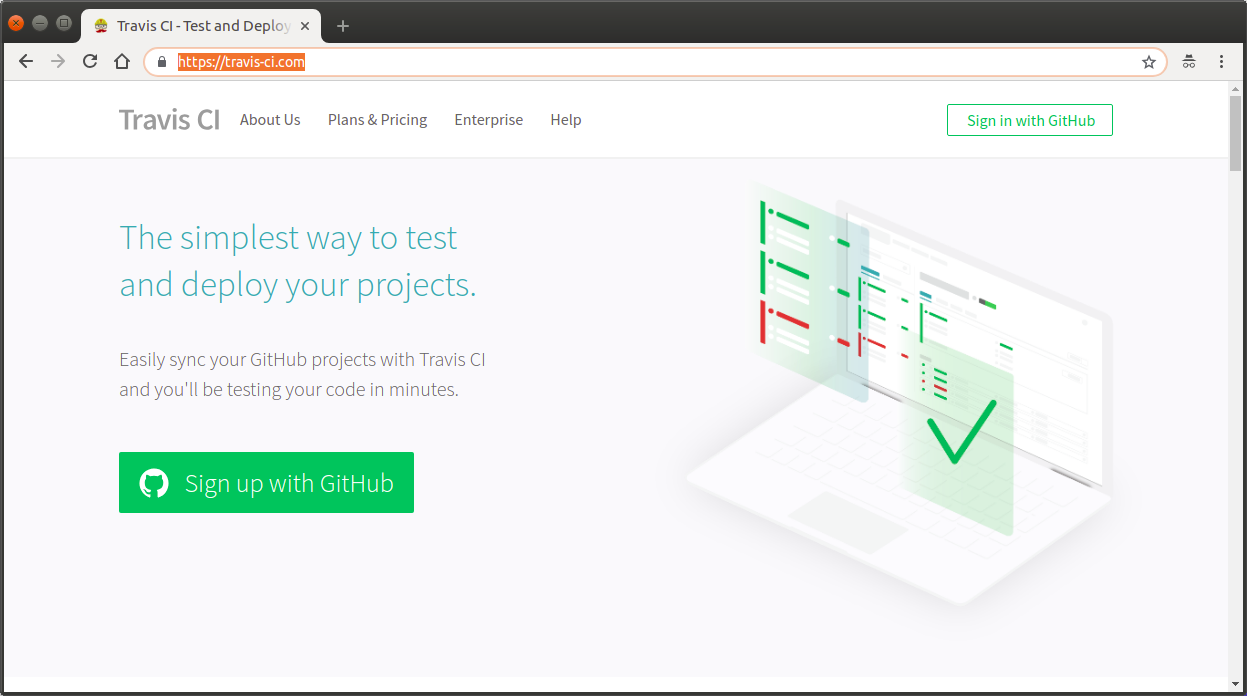
\includegraphics[width=4.5in]{\thischapterpath/figures/travis01.png}}
\caption{Travis-CI.com is a website supporting continuous integration.}
\label{fig:travis01}
\end{figure}

\index{pytest|)}
